\documentclass[11pt]{article}
\title{\textbf{CS 361 Spring 2018\\Homework 9}}
\author{Nathaniel Murphy (njmurph3)}
\date{}

\usepackage{a4wide}
\usepackage{amsfonts}
\usepackage{amsmath}
\usepackage{amsthm}
\usepackage{graphicx}
\usepackage[margin=0.5in]{geometry}

\newcommand{\given}{\hspace{1mm}|\hspace{1mm}}
\newcommand{\hsp}{\hspace{1mm}}
\newcommand{\mean}{\text{mean}}
\newcommand{\var}{\text{var}}

\begin{document}
\maketitle
\section*{10.1}
\subsection*{(a)}
\[\text{mean}(\{f\})=\text{mean}(a^T\{x\})\]
\[=a^T\text{mean}(\{x\}\]
because $a^T$ is a constant.
\subsection*{(b)}
\[\var(\{f\})=\var(a^T\{x\})\]
\[=\frac{\sum_i\left(a^Tx_i-\mean(a^T\{x\})\right)\left(a^Tx_i-\mean(a^T\{x\})\right)^T}{N}\]
\[=\frac{\sum_i\left(a^Tx_i-a^T\mean(\{x\})\right)\left(a^Tx_i-a^T\mean(\{x\})\right)^T}{N}\]
\[=\frac{\sum_i\left(a^T(x_i-\mean(\{x\})\right)\left(a^T(x_i-\mean(\{x\})\right)^T}{N}\]
\[=\frac{\sum_ia^T(x_i-\mean(\{x\}))(x_i-\mean(\{x\}))^Ta}{N}\hspace{7mm}\text{ because }(AB)^T=B^TA^T\]
\[=a^T\left(\frac{\sum_i(x_i-\mean(\{x\}))(x_i-\mean(\{x\}))^T}{N}\right)a\]
\[=a^T\text{Covmat}(\{x\})a\]
\subsection*{(c)}
Suppose that for some $a$, $a^T$Covmat$(\{x\})a=0$. \\ \\
Because $a^T$Covmat$(\{x\})a=0$, we know that $a^T$ is an eigenvector of Covmat$(\{x\})$ with eigenvalue 0. because the eigenvalue is 0, we can say that this eigenvector preserves no variance of the data. Consider the hyperplane that is orthogonal to $a^T$. this hyperplane must preserve all variance of the data simply by the fact that $a^T$ preserves non. Since 100\% of the data can be expressed with this hyperplan, it must follow that the dataset lies in a hyperplane.
\clearpage
\section*{10.2}
\begin{figure}[h!]
	\centering
	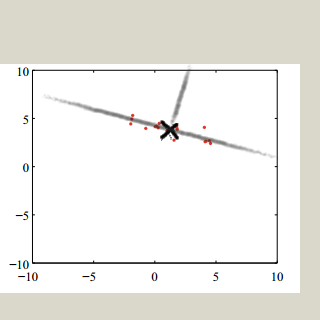
\includegraphics[width=100mm]{10_2.png}
\end{figure}
\ \\
The black X drawn on the data represents the mean of the dataset. The longer horizontal line represents the first principle component because most of the variance lies on this line. Finally, the second principle component is perpendicular to the first principle component and this represents the variance not captured by the first principle component.
\clearpage
\section*{10.3}
\subsection*{(a)}
Because the covariance matrix has one non-zero eigenvalue, we may say that 100\% of the variance of the data can be explained using one dimension. This implies that all of the data points lie on a line in d-dimensional space. This means that any data point is a basis for the data set. i.e.
\[x_i=a\cdot x_j\text{ for some }a\in\mathbb{R}\text{ and }j<N\]
It clearly follows that
\[x_i=a\cdot x_j\Rightarrow x_i = x_1 + t_i(x_2-x_1)\]
because $x_2-x_1$ lies on the same line formed by $x_1$ and $x_2$ continuing infinitely (because they are linearly dependent). Call this value $x_k$. $x_k-x_1$ is also on the infinite line formed by $x_1$ and $x_2$ because of the same linear dependence between all vectors in the dataset. Let $x_\ell=x_k-x_1$. Because the infinite line formed by $x_1$ and $x_2$ si precisely $a\cdot x_j$, $a\in\mathbb{R}$, $j<N$, we can say that such an $a\in\mathbb{R}$ exists such that $x_i=a\cdot x_\ell$.
\subsection*{(b)}
Because all the variance is explained using 1 dimension, the $t$ values are precisely the dataset projected on the line $a\cdot x_j$, $a\in\mathbb{R}$, $j<N$. Because no variance is lost, std$(\{t\})=$std$(\{x\})$.
\clearpage
\begin{figure}[h!]
	\centering
	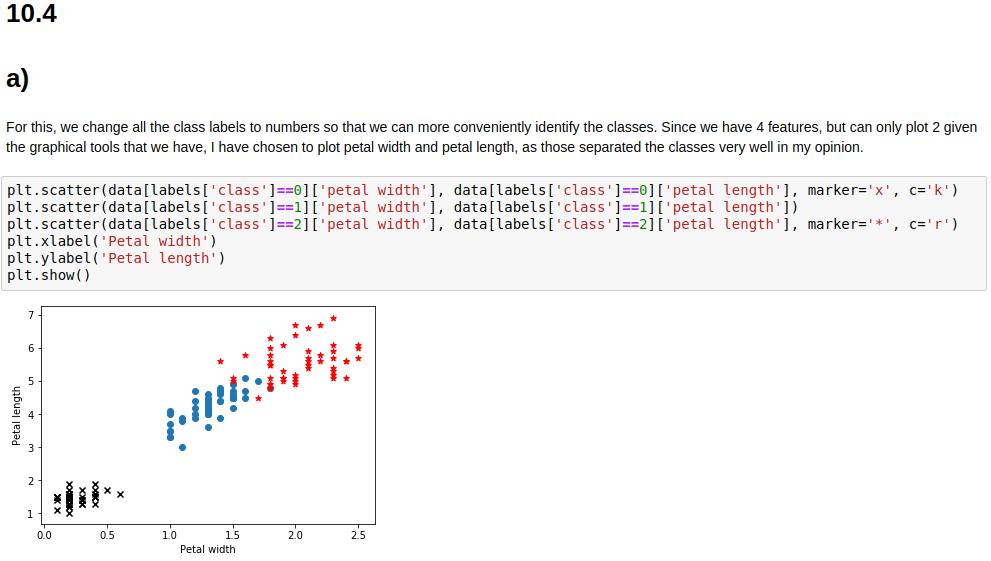
\includegraphics[width=200mm]{10_4a.png}
\end{figure}
\clearpage
\begin{figure}[h!]
	\centering
	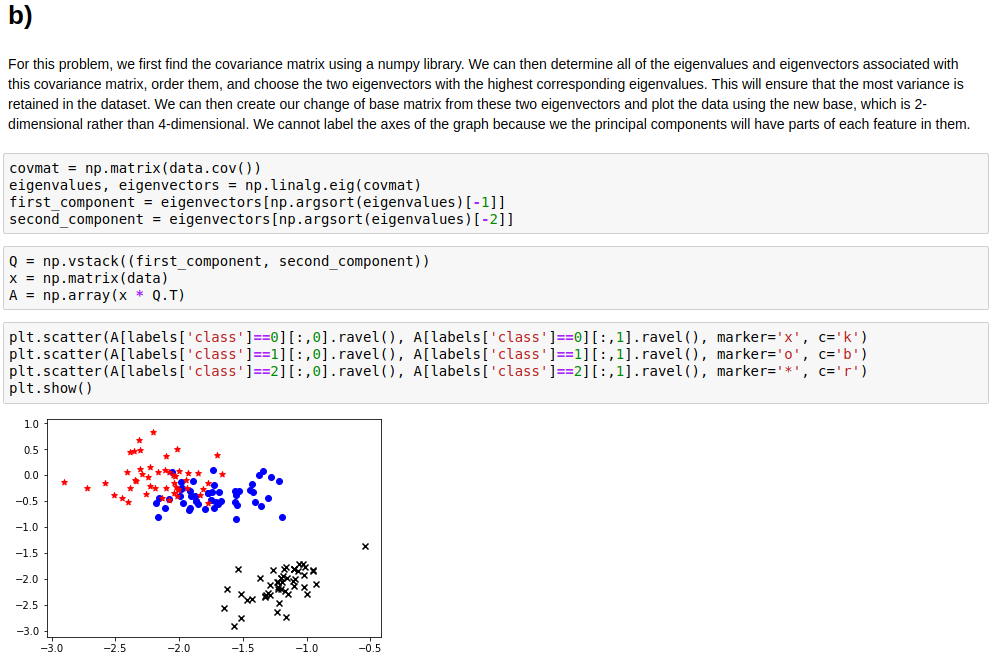
\includegraphics[width=200mm]{10_4b.png}
\end{figure}
\clearpage
\begin{figure}[h!]
	\centering
	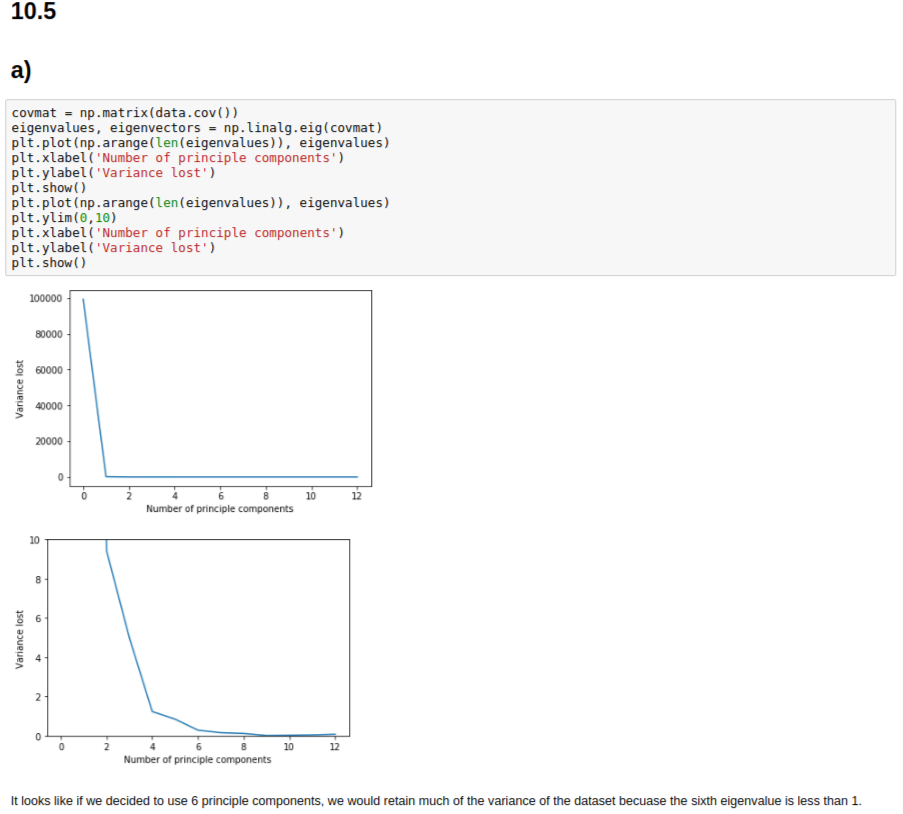
\includegraphics[width=200mm]{10_5a.png}
\end{figure}
\clearpage
\begin{figure}[h!]
	\centering
	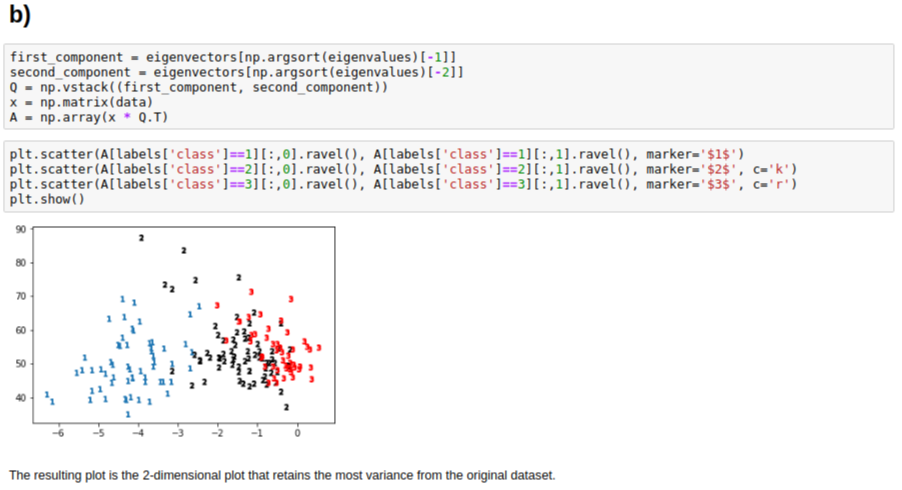
\includegraphics[width=200mm]{10_5b.png}
\end{figure}
\clearpage
\begin{figure}[h!]
	\centering
	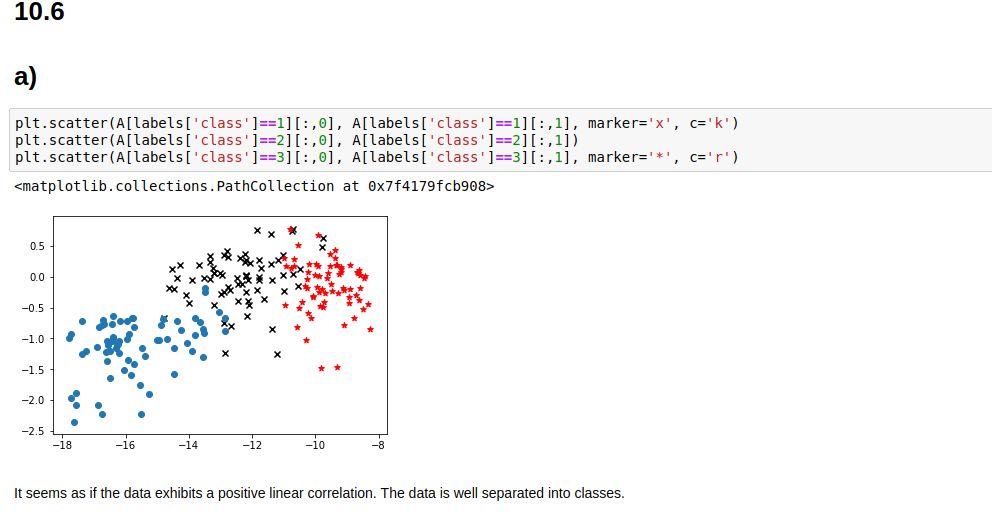
\includegraphics[width=200mm]{10_6a.png}
\end{figure}
\begin{figure}[h!]
	\centering
	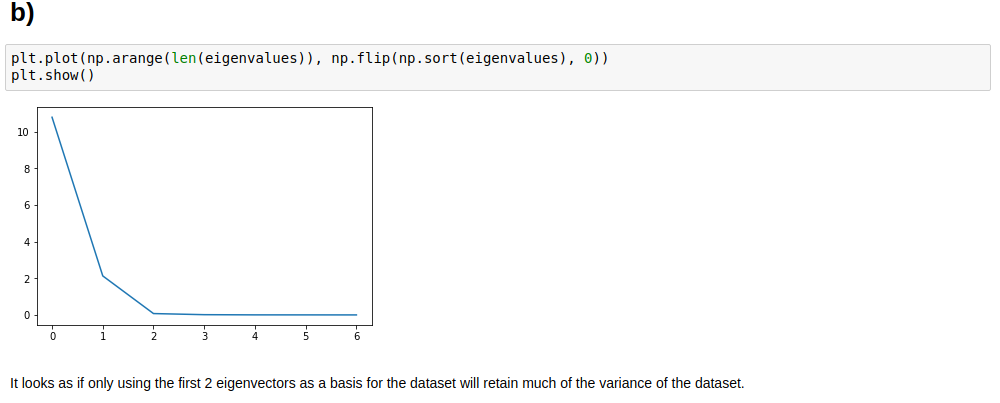
\includegraphics[width=200mm]{10_6b.png}
\end{figure}
\end{document}





